\documentclass{article}

% packages
\usepackage[margin=.5in]{geometry}
\usepackage{pdflscape}
\usepackage{amsmath,amssymb}
\usepackage{newtx,newtxmath}
\usepackage[none]{hyphenat}
\usepackage{calc}
\usepackage{enumitem}
\usepackage{float}
\usepackage{pgffor}
\usepackage{multirow}
\usepackage[dvipsnames]{xcolor}
\usepackage{hyperref}
\usepackage{tikz}

% details
\author{koku17}
\title{Theory of Computation}

% ricing
\def \darkmode{1}
\if\darkmode1
	\pagecolor{black}
	\color{white}
\fi
\definecolor{BrightGreen}{rgb}{.4, 1, 0}
\def \hltt{\color{BrightGreen}}

% presets
\hypersetup{
    hidelinks
}
\usetikzlibrary{
	automata,
	positioning,
	arrows.meta
}

\tikzset{
	node distance=5em,
	every loop/.append style={
		-Straight Barb
	},
	every initial by arrow/.style={
		-Straight Barb
	},
	every edge/.append style={
		-Straight Barb
	},
	initial text=
}

\if\darkmode1
	\tikzset{double=black}
\fi

% macros
\def \mds{\displaystyle}
\newcommand{\module}[1]{
	 
	\item[] \phantomsection \begin{center} {\LARGE Module #1} \end{center}
	\addcontentsline{toc}{section}{Module #1}
}

\def \answer{\item [$\rightarrow$]}
\def \indentpar#1#2{
    \begin{itemize}[leftmargin=#1,label=]
        \item #2
    \end{itemize}
}

\newlength{\ansindent}
\setlength{\ansindent}{\widthof{\phantom{$\longrightarrow$}}}

\def \OR{\item [] \hfill OR \hfill~\!}
\def \DFA{Deterministic Finite Automata}
\def \DFSM{Deterministic Finite State Machine}
\def \REGEX{Regular Expression}

\begin{document}
    \pagenumbering{gobble} \maketitle \newpage
    \pagenumbering{roman} \pdfbookmark[1]{Contents}{} \tableofcontents \newpage
    \pagenumbering{arabic}

	\begin{itemize}
		\module{1}
		\item [1a.] Obtain a DFA to accept strings of a’s and b’s having odd number of a’s and even number of
			b’s.
		\answer
			\begin{enumerate}[label=Step \arabic* :,itemindent=\ansindent]
				\item Identify the number of states
				\indentpar{1.5em}{
					Since Even numbers can be 0 and multiple of 2 for 2 letters, there are 4 different states :
					\begin{itemize}[leftmargin=1.5em]
						\item Both $a$'s and $b$'s are even i.e $\text{E}_a\text{E}_b$
						\item Even $a$'s and odd $b$'s i.e $\text{E}_a\text{O}_b$
						\item Odd $a$'s and even $b$'s i.e $\text{O}_a\text{E}_b$
						\item Both $a$'s and $b$'s are odd i.e $\text{O}_a\text{O}_b$
					\end{itemize}
				}
				\item Identify the initial and accepting states
					\begin{itemize}[leftmargin=2.5em]
						\item In case of 0 or multiple of 2 input the state is accepted.
						\item All the rest of the cases are rejected.
					\end{itemize}
				\item Complete Transitions
					\begin{table}[H]
						\centering
						\begin{tabular}{cc}
							\begin{tabular}{c|c|c}
								$\delta$ & $a$ & $b$ \\ \hline
								$\text{E}_a\text{E}_b$ & $\text{O}_a\text{E}_b$ & $\text{E}_a\text{O}_b$ \\
								$\text{O}_a\text{E}_b$ & $\text{E}_a\text{E}_b$ & $\text{O}_a\text{O}_b$ \\
								$\text{E}_a\text{O}_b$ & $\text{O}_a\text{O}_b$ & $\text{E}_a\text{E}_b$ \\
								$\text{O}_a\text{O}_b$ & $\text{E}_a\text{O}_b$ & $\text{O}_a\text{E}_b$
							\end{tabular}
							\begin{tabular}{lll}
								$\delta(\text{E}_a\text{E}_b,a)$ & $=$ & $\text{O}_a\text{E}_b$ \\
								$\delta(\text{E}_a\text{E}_b,b)$ & $=$ & $\text{E}_a\text{O}_b$ \\
								$\delta(\text{O}_a\text{E}_b,a)$ & $=$ & $\text{E}_a\text{E}_b$ \\
								$\delta(\text{O}_a\text{E}_b,b)$ & $=$ & $\text{O}_a\text{O}_b$ \\
								$\delta(\text{E}_a\text{O}_b,a)$ & $=$ & $\text{O}_a\text{E}_b$ \\
								$\delta(\text{E}_a\text{O}_b,b)$ & $=$ & $\text{E}_a\text{E}_b$ \\
								$\delta(\text{O}_a\text{O}_b,b)$ & $=$ & $\text{E}_a\text{O}_b$ \\
								$\delta(\text{O}_a\text{O}_b,b)$ & $=$ & $\text{O}_a\text{E}_b$
							\end{tabular}
						\end{tabular}
					\end{table}
				\item Final Design \def \tn#1#2{node[draw=white,minimum width=#1,minimum height=#2]}
\def \trn#1#2#3{node[#1,draw=white,minimum width=#2,minimum height=#3]}

\begin{figure}[H]
	\centering
	\begin{tikzpicture}[node distance=5em]
		\draw
			\tn{5em}{2em} (u) {User}
			\trn{below of=u}{5em}{2em} (sh) {Shell}
			\trn{below of=sh,xshift=-10em}{5em}{2em} (ut) {Utilities}
			\trn{below of=sh,xshift=10em}{5em}{2em} (ap) {
				\begin{tabular}{c}Application \\ Program\end{tabular}
			}
			\trn{below of=sh,yshift=-5em}{5em}{2em} (k) {Kernel}
			\trn{below of=k}{5em}{2em} (h) {Hardware}

		;
		\draw[-Straight Barb] (u) -- (sh);
		\draw[-Straight Barb](sh) -| (ut);
		\draw[-Straight Barb](sh) -| (ap);
		\draw[-Straight Barb](sh) -- (k);
		\draw[-Straight Barb](k) -- (h);
	\end{tikzpicture}
\end{figure}

			\end{enumerate}
		\newpage

		\item [1b.] Draw a DFA to accept decimal strings divisible by 3
		\answer
						\begin{enumerate}[label=Step \arabic* :,itemindent=\ansindent]
				\item Identify the radix, input alphabets and the divisor
					\begin{align*}
						r&=10 \\
						d&=\{0,1,2,3,4,5,6,7,8,9\} \\
						k&=3
					\end{align*}
				\item Compute Possible remainders \\ $i=\{0,1,2\}$
				\item Compute Transitions
					\begin{table}[H]
						\centering
						\begin{tabular}{cc}
							\begin{tabular}{|c|c|c|c|} \hline
								$i$ & $d$ & $j$ & $\delta(q_i,d)=q_j$ \\ \hline
								\multirow{3}*{0} & 0 & 0 & $\delta(q_0,0)=q_0$ \\ \cline{2-4}
									& 1 & 1 & $\delta(q_0,1)=q_1$ \\ \cline{2-4}
									& 2 & 2 & $\delta(q_0,2)=q_2$ \\ \hline
								\multirow{3}*{1} & 0 & 1 & $\delta(q_1,0)=q_1$ \\ \cline{2-4}
									& 1 & 2 & $\delta(q_1,1)=q_2$ \\ \cline{2-4}
									& 2 & 0 & $\delta(q_1,2)=q_0$ \\ \hline
								\multirow{3}*{2} & 0 & 2 & $\delta(q_2,0)=q_2$ \\ \cline{2-4}
									& 1 & 0 & $\delta(q_2,1)=q_0$ \\ \cline{2-4}
									& 2 & 1 & $\delta(q_2,2)=q_1$ \\ \hline
								\multirow{3}*{3} & 0 & 0 & $\delta(q_3,0)=q_0$ \\ \cline{2-4}
									& 1 & 1 & $\delta(q_3,1)=q_1$ \\ \cline{2-4}
									& 2 & 2 & $\delta(q_3,2)=q_2$ \\ \hline
							\end{tabular} &
							\begin{tabular}{lll}
								$\delta(q_0,\{0,3,6,9\})$ & $=$ & $q_0$ \\
								$\delta(q_0,\{1,4,7\})$   & $=$ & $q_1$ \\
								$\delta(q_0,\{2,5,8\})$   & $=$ & $q_2$ \\
								$\delta(q_1,\{0,3,6,9\})$ & $=$ & $q_1$ \\
								$\delta(q_1,\{1,4,7\})$   & $=$ & $q_2$ \\
								$\delta(q_1,\{2,5,8\})$   & $=$ & $q_0$ \\
								$\delta(q_2,\{0,3,6,9\})$ & $=$ & $q_2$ \\
								$\delta(q_2,\{1,4,7\})$   & $=$ & $q_0$ \\
								$\delta(q_2,\{2,5,8\})$   & $=$ & $q_1$
							\end{tabular} \\ ~\vspace{-.5em} \\
							Transitions & Counter DFA
						\end{tabular}
					\end{table}
				\item Final DFA
					\input{QP/1b.tikz}
			\end{enumerate}
		\newpage

		\item [1c.] Define the following terms with example:
			\begin{enumerate}[label=\roman*)]
				\item Alphabet
				\item Power of Alphabet
				\item Languages
			\end{enumerate}
		\answer
			\begin{enumerate}[label=\roman*)]
				\item Alphabet
					\begin{itemize}
						\item It is a finite, non-empty set of symbols.
						\item It is denoted by $\sum$
						\item Example
							\begin{enumerate}[label=\alph*)]
								\item $\sum=\{0,1\}$, the binary alphabet
								\item $\sum=\{a,b,\cdots,z\}$, the set of all lowercase letters
							\end{enumerate}
					\end{itemize}
				\item Power of Alphabet
					\begin{itemize}
						\item The power of an alphabet is denoted by $\sum^i$
						\item $\sum^n=\sum^0\bigcup\sum^1\bigcup\sum^2\bigcup\sum^3\cdots\bigcup\sum^n$
							(include empty string)
						\item $\sum^n=\sum^1\bigcup\sum^2\bigcup\sum^3\cdots\bigcup\sum^n$
							(exclude empty string)
						\item Example
							\begin{enumerate}[label=\alph*)]
								\item $\sum^0=\{\varepsilon\}-$ set of word length is 0
								\item $\sum^i=\{0,1\}$, $\{a,b,c\}-$ set of word length is 1
								\item $\sum^2=\{00,01,11,10\}$, $\{aa,ab,bb,ba\}-$ set of word length is 2
								\item $\sum^3=\{000,001,010,100,011,110,111\}-$ set of word length is 3
							\end{enumerate}
					\end{itemize}
				\item Languages
					\begin{itemize}
						\item It is the set of strings obtained from $\sum^n$, where $\sum$ is the set of
							alphabets of particular language
						\item Example
							\begin{enumerate}[label=\alph*)]
								\item L$_1=\{w^2|w\in(0,1)\}$, set of all strings of length 2
								\item L$_2=\{w^3|w\in(0,1)\}$, set of all strings of length 3
								\item L$_3=\{|w\in(0,1)\}$, set of all strings of length 3
							\end{enumerate}
					\end{itemize}
			\end{enumerate}
		\OR
		\item [2a.] Obtain an $\varepsilon$-NFA which accepts strings consisting of zero or more a’s followed by
			zero or more b’s followed by zero or more c’s.
		\answer ~\begin{figure}[H]
	\centering
	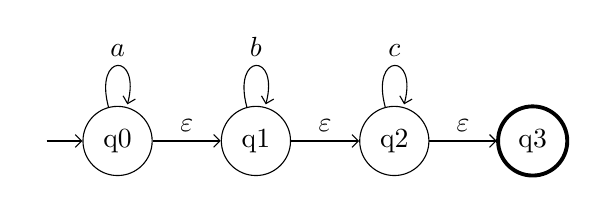
\begin{tikzpicture}
		\draw
			node [state,initial]               (q0) {q0}
			node [state,right of=q0]           (q1) {q1}
			node [state,right of=q1]           (q2) {q2}
			node [state,right of=q2,accepting] (q3) {q3}
	
			\foreach[count=\j] \i in {0,...,3} {
				\ifnum4>\j
					(q\i) edge[above] node {$\varepsilon$} (q\j)
				\fi
				\ifnum3>\i
					(q\i) edge[loop above] node {$\char\the\numexpr97+\i\relax$} (q\i)
				\fi
			}
		;
	\end{tikzpicture}
\end{figure}

			Where,
			\begin{itemize}
				\item $q_0 \rightarrow$ accept zero or more $a$'s
				\item $q_1 \rightarrow$ accept zero or more $b$'s
				\item $q_2 \rightarrow$ accept zero or more $c$'s
				\item $q_3 \rightarrow$ accepting state
				\item $\varepsilon-$ closure $(q_0)=\{q_0,q_1,q_2,q_3\}$
				\item $\varepsilon-$ closure $(q_1)=\{q_0,q_2,q_3\}$
				\item $\varepsilon-$ closure $(q_2)=\{q_2,q_3\}$
				\item $\varepsilon-$ closure $(q_3)=\{q_3\}$
			\end{itemize}
		\newpage

		\item [2b.] Define Deterministic Finite Automata. \\
			Explain the two preferred notations for describing the Transition Function with an example.
		\answer \DFA is quintuple indicating 5 components $$\text{M}=(\text{Q},\sum,\delta,q_0,\text{F})$$
			Where,
			\begin{enumerate}
				\item [Q $\rightarrow$] Finite set of states
				\item [$\sum\rightarrow$] Finite set of input symbols
				\item [$\delta\rightarrow$] Transitions from $(\text{Q}\times\sum)\to \text{Q}$
				\item [$q_0\rightarrow$] Initial state
				\item [F$\rightarrow$] Set of accepting states
			\end{enumerate}
		\textbf{Notations of DFA}
		\begin{enumerate}
			\item Transition Diagram
				\begin{itemize}
					\item A graph which shows states and input of a \DFSM to represent a Transition function.
					\item Example \begin{figure}[H]
	\centering
	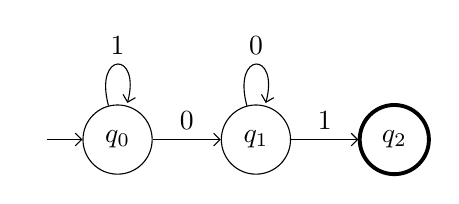
\begin{tikzpicture}
		\draw
			node[initial,state]               (q0) {$q_0$}
			node[state,right of=q0]           (q1) {$q_1$}
			node[state,right of=q1,accepting] (q2) {$q_2$}
			
			(q0) edge[loop above] node {1} (q0)
			(q1) edge[loop above] node {0} (q1)
			(q0) edge[above] node {0} (q1)
			(q1) edge[above] node {1} (q2)
		;
	\end{tikzpicture} \\
	Accepting all strings with substring 01
\end{figure}

				\end{itemize}
			\item Transition Table
				\begin{itemize}
					\item A table which shows transitions of input of a \DFSM to represent a Transition function.
					\item Example
						\begin{table}[H]
							\centering
							\begin{tabular}{c|c|c}
								$\delta$ & 0 & 1 \\ \hline
								$q_0$ & $q_1$ & $q_0$ \\
								$q_1$ & $q_1$ & $q_0$ \\
								$q_2$ & $q_2$ & $q_2$
							\end{tabular} \\ ~ \\
							Transition table for the above graph
						\end{table}
				\end{itemize}
		\end{enumerate}
	\item [2c.] Obtain a DFA for the following NFA using lazy evaluation method. \begin{figure}[H]
	\centering
	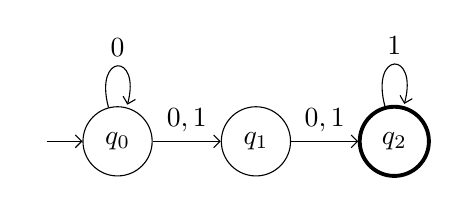
\begin{tikzpicture}
		\draw
			node[state,initial]               (q0) {$q_0$}
			node[state,right of=q0]           (q1) {$q_1$}
			node[state,right of=q1,accepting] (q2) {$q_2$}

			(q0) edge[loop above] node{$0$}   (q0)
			(q2) edge[loop above] node{$1$}   (q2)
			(q0) edge[above]      node{$0,1$} (q1)
			(q1) edge[above]      node{$0,1$} (q2)
		;
	\end{tikzpicture}
\end{figure}

	\answer
		\begin{enumerate}[label=Step \arabic* :,itemindent=\ansindent]
			\item Find Transitions
				\begin{table}[H]
					\centering
					\begin{tabular}{c|c|c}
						$\delta$ & 0             & 1     \\ \hline
						$q_0$    & $\{q_0,q_1\}$ & $q_1$ \\
						$q_1$    & $q_2$         & $q_2$ \\
						$q_2$    & $\varnothing$ & $q_2$
					\end{tabular}
				\end{table}
			\item Identify initial and accepting state
				\begin{itemize}[label=,leftmargin=1.5em]
					\item $\text{F}_0=\{q_2,\{q_0,q_2\},\{q_0,q_1,q_2\}\}$
					\item $\text{F}_1=q_2$
				\end{itemize}
			\item Identify transitions for all possible subsets
				\begin{table}[H]
					\centering
					\begin{tabular}{cc}
						\begin{tabular}{c|c|c}
							$\delta$          & 0                 & 1             \\ \hline
							$q_0$             & $\{q_0,q_1\}$     & $q_1$         \\
							$q_1$             & $q_2$             & $q_2$         \\
							$q_2$             & $\varnothing$     & $q_2$         \\
							$\{q_0,q_1\}$     & $\{q_0,q_1,q_2\}$ & $\{q_1,q_2\}$ \\
							$\{q_1,q_2\}$     & $q_2$             & $q_2$         \\
							$\{q_0,q_2\}$     & $\{q_0,q_1\}$     & $\{q_1,q_2\}$ \\
							$\{q_0,q_1,q_2\}$ & $\{q_0,q_1,q_2\}$ & $\{q_1,q_2\}$
						\end{tabular} &
						\begin{tabular}{ccc}
							$\delta(q_0,0)$             & $=$ & $\{q_0,q_1\}$     \\
							$\delta(q_0,1)$             & $=$ & $q_1$             \\
							$\delta(q_1,0)$             & $=$ & $q_2$             \\
							$\delta(q_1,1)$             & $=$ & $q_2$             \\
							$\delta(q_2,1)$             & $=$ & $q_2$             \\
							$\delta(\{q_0,q_1\},0)$     & $=$ & $\{q_0,q_1,q_2\}$ \\
							$\delta(\{q_0,q_1\},1)$     & $=$ & $\{q_1,q_2\}$     \\
							$\delta(\{q_1,q_2\},0)$     & $=$ & $q_2$             \\
							$\delta(\{q_1,q_2\},1)$     & $=$ & $q_2$             \\
							$\delta(\{q_0,q_2\},0)$     & $=$ & $\{q_0,q_1\}$     \\
							$\delta(\{q_0,q_2\},1)$     & $=$ & $\{q_1,q_2\}$     \\
							$\delta(\{q_0,q_1,q_2\},0)$ & $=$ & $\{q_1,q_2\}$     \\
							$\delta(\{q_0,q_1,q_2\},1)$ & $=$ & $\{q_1,q_2\}$
						\end{tabular}
					\end{tabular}
				\end{table}
			\item Convert transitions to DFA
				\indentpar{1.5em}{Replace Similar elements with a letter}
				\begin{table}[H]
					\centering
					\begin{tabular}{c|c|c}
						$\delta$          & 0                       & 1                   \\ \hline
				\hltt	$q_0$             & $\{q_0,q_1\}$           & $q_1$               \\
				\hltt	$\{q_0,q_1\}$     & $\{q_0,q_1,q_2\}$       & $\{q_1,q_2\}$       \\
				\hltt	$q_1$             & $q_2$                   & $q_2$               \\
				\hltt	$\{q_0,q_1,q_2\}$ & \hltt $\{q_0,q_1,q_2\}$ & \hltt $\{q_1,q_2\}$ \\
				\hltt	$\{q_1,q_2\}$     & \hltt $q_2$             & \hltt	$q_2$         \\
				\hltt	$q_2$             & $\varnothing$           & \hltt	$q_2$
					\end{tabular}
				\end{table}
			\item Final DFA \begin{figure}[H]
	\centering
	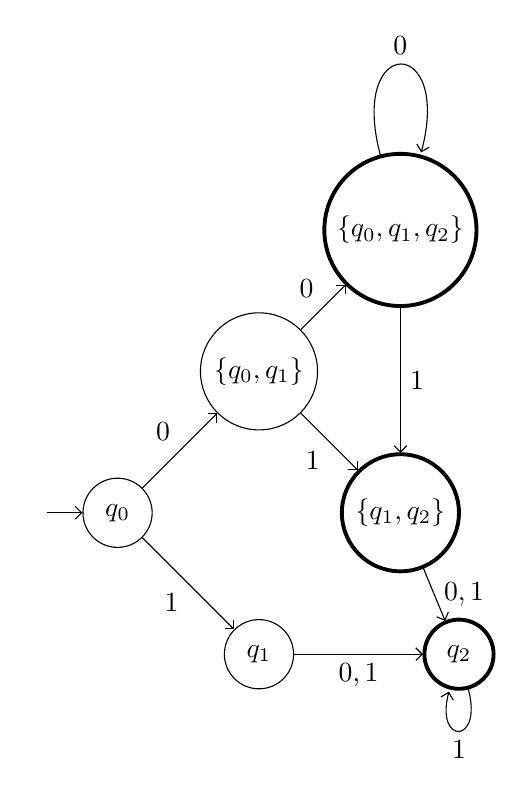
\begin{tikzpicture}[node distance=1in]
		\draw
			node[state,initial]                       (q0)     {$q_0$}
			node[state,above right of=q0]             (q0q1)   {$\{q_0,q_1\}$}
			node[state,below right of=q0]             (q1)     {$q_1$}
			node[state,accepting,above right of=q0q1] (q0q1q2) {$\{q_0,q_1,q_2\}$}
			node[state,accepting,below right of=q0q1] (q1q2)   {$\{q_1,q_2\}$}
			node[state,accepting,right of=q1]         (q2)     {$q_2$}

			(q0) edge[above left] node {0} (q0q1)
			(q0) edge[below left] node {1} (q1)
			(q0q1) edge[above left] node {0} (q0q1q2)
			(q0q1) edge[below left] node {1} (q1q2)
			(q0q1q2) edge[loop above] node {0} (q0q1q2)
			(q0q1q2) edge[right] node {1} (q1q2)
			(q1q2) edge[right] node {$0,1$} (q2)
			(q1) edge[below] node {$0,1$} (q2)
			(q2) edge[loop below] node {$1$} (q2)
		;
	\end{tikzpicture}
\end{figure}

		\end{enumerate} \newpage

		\module{2}
		\item[3a.] List applications of RE.
			What are the notations used in UNIX Operation system ? \\
			List few Regular expressions with its UNIX notations.
		\answer
			\begin{enumerate}
				\item Lexical analysis \\
					\REGEX s are used to define token by matching valued lexers for token
					categorization in languages like C
				\item Web Development \\
					\REGEX s are used in web development for tasks like URL routing, form validation and
					extraction data from HTML/XML document.
				\item Data validation \\
					\REGEX~are used to validate user input such as email addresses, phone numbers and passwords
				\item Extracting data \\
					\REGEX~can be used to extract data from Structured or semi-structured text as names,
					addresses or dates.
				\item Search \& Replace \\
					\REGEX~cache used to find specific pattern in text \& replace them with desired text
			\end{enumerate}
		\textbf{\REGEX~in UNIX} \\
		A regular expression is a set of characters that specify a pattern
		\begin{itemize}[itemindent=1em]
			\item [\texttt{$\cdot$}] A dot will match any single character except a newline character
			\item [\texttt{*,+}] Star or plus are used to match zero/one or more of the preceding expressions
			\item [\texttt{?}] Matches zero or one copy of the preceding expression
			\item [\texttt{|}] A logical `or' statement - matches either the pattern before it, or the pattern
				after
			\item [\texttt{\textasciicircum}] Matches the very beginning of a line
			\item [\texttt{\$}] Matched the end of a line
			\item [\texttt{/}] Matches the preceding regular expression, but only if followed by the subsequent
				expression
			\item [$\texttt{[]}$] Brackets are used to denote a character class, which matches any single
				character within the brackets
			\item [\texttt{""}] Match everything within the quotes literally
			\item [\texttt{()}] Group everything in the parentheses as a single unit for the rest of the
				expression
		\end{itemize}
		\newpage

		\item[3b.] Obtain an $\varepsilon$-NFA for the Regular Expression $(a+b)*~bb~(a+b)*$
		\answer
			\begin{enumerate}[label=Step \arabic* :,itemindent=\ansindent]
				\item $\varepsilon$-NDFA for $a+b$ \begin{figure}[H]
	\centering
	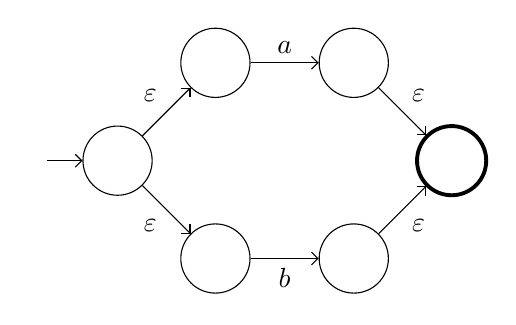
\begin{tikzpicture}
		\draw
			node[initial,state]                    (1) {~}
			node[state,above right of=1]           (2) {~}
			node[state,right of=2]                 (3) {~}
			node[state,below right of=3,accepting] (4) {~}
			node[state,below right of=1]           (5) {~}
			node[state,right of=5]                 (6) {~}

			(1) edge[above left]  node {$\varepsilon$} (2)
			(2) edge[above]       node {$a$} (3)
			(3) edge[above right] node {$\varepsilon$} (4)
			(1) edge[below left]  node {$\varepsilon$} (5)
			(5) edge[below]       node {$b$} (6)
			(6) edge[below right] node {$\varepsilon$} (4)
		;
	\end{tikzpicture}
\end{figure}

				\item $\varepsilon$-NDFA for $(a+b)^*$ \begin{figure}[H]
	\centering
	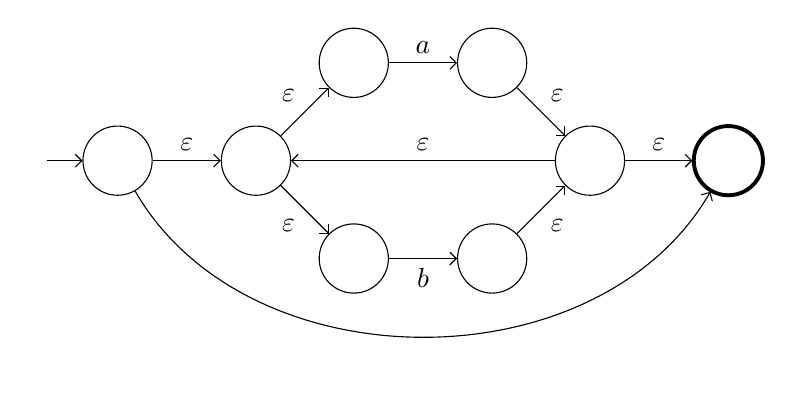
\begin{tikzpicture}
		\draw
			node[initial,state]              (0) {~}
			node[state,right of=0]           (1) {~}
			node[state,above right of=1]     (2) {~}
			node[state,right of=2]           (3) {~}
			node[state,below right of=3]     (4) {~}
			node[state,below right of=1]     (5) {~}
			node[state,right of=5]           (6) {~}
			node[state,right of=4,accepting] (7) {~}

			(0) edge[above]               node {$\varepsilon$} (1)
			(1) edge[above left]          node {$\varepsilon$} (2)
			(2) edge[above]               node {$a$} (3)
			(3) edge[above right]         node {$\varepsilon$} (4)
			(1) edge[below left]          node {$\varepsilon$} (5)
			(5) edge[below]               node {$b$} (6)
			(6) edge[below right]         node {$\varepsilon$} (4)
			(4) edge[above]               node {$\varepsilon$} (7)
			(4) edge[above]               node {$\varepsilon$} (1)
			(0) edge[below,bend right=60] node {~} (7)
		;
	\end{tikzpicture}
\end{figure}

				\item $\varepsilon$-NDFA for $(a+b)^*~bb$ \input{QP/3b.3.tikz}
				\begin{landscape}
					\thispagestyle{empty}
					\item $\varepsilon$-NDFA for $(a+b)^*~bb~(a+b)^*$ \begin{figure}[H]
	\centering
	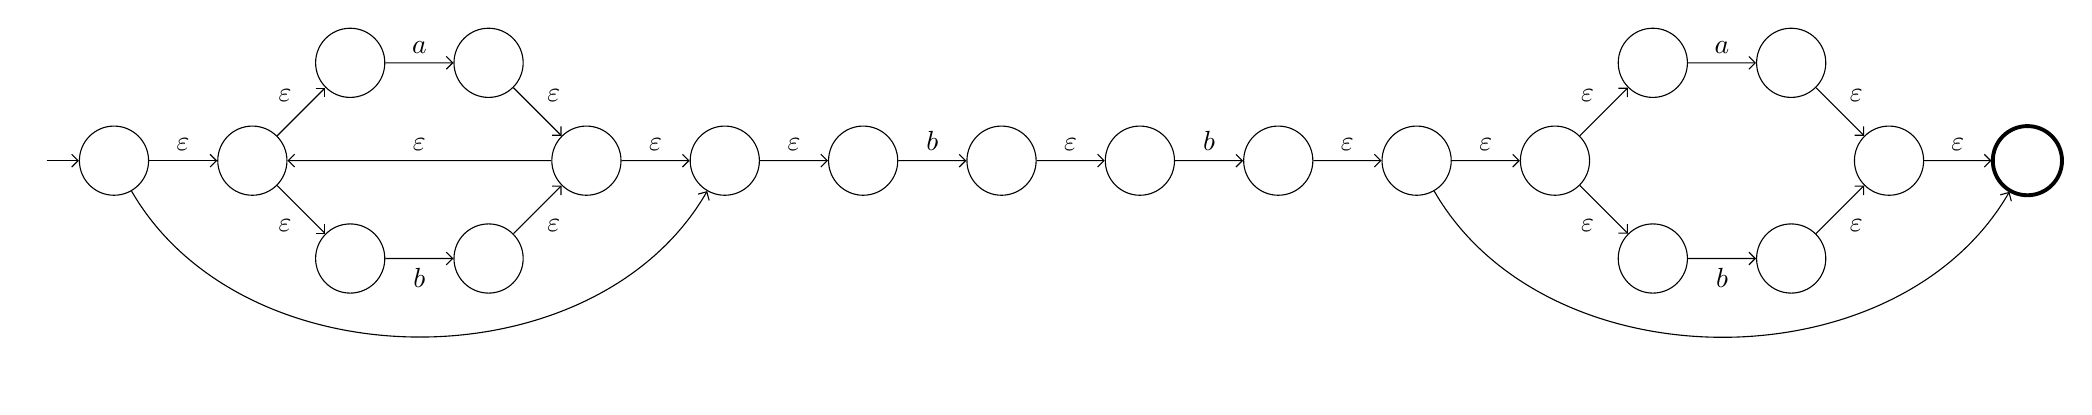
\begin{tikzpicture}[scale=.9]
		\draw
			node[initial,state]               (0)  {~}
			node[state,right of=0]            (1)  {~}
			node[state,above right of=1]      (2)  {~}
			node[state,right of=2]            (3)  {~}
			node[state,below right of=3]      (4)  {~}
			node[state,below right of=1]      (5)  {~}
			node[state,right of=5]            (6)  {~}
			node[state,right of=4]            (7)  {~}
			node[state,right of=7]            (8)  {~}
			node[state,right of=8]            (9)  {~}
			node[state,right of=9]            (10) {~}
			node[state,right of=10]           (11) {~}
			node[state,right of=11]           (12) {~}
			node[state,right of=12]           (13) {~}
			node[state,above right of=13]     (14) {~}
			node[state,right of=14]           (15) {~}
			node[state,below right of=15]     (16) {~}
			node[state,below right of=13]     (17) {~}
			node[state,right of=17]           (18) {~}
			node[state,right of=16,accepting] (19) {~}

			(0)  edge[above]               node {$\varepsilon$} (1)
			(1)  edge[above left]          node {$\varepsilon$} (2)
			(2)  edge[above]               node {$a$}           (3)
			(3)  edge[above right]         node {$\varepsilon$} (4)
			(1)  edge[below left]          node {$\varepsilon$} (5)
			(5)  edge[below]               node {$b$}           (6)
			(6)  edge[below right]         node {$\varepsilon$} (4)
			(4)  edge[above]               node {$\varepsilon$} (7)
			(4)  edge[above]               node {$\varepsilon$} (1)
			(0)  edge[below,bend right=60] node {~}             (7)
			(7)  edge[above]               node {$\varepsilon$} (8)
			(8)  edge[above]               node {$b$}           (9)
			(9)  edge[above]               node {$\varepsilon$} (10)
			(10) edge[above]               node {$b$}           (11)
			(11) edge[above]               node {$\varepsilon$} (12)
			(12) edge[above]               node {$\varepsilon$} (13)
			(13) edge[above left]          node {$\varepsilon$} (14)
			(14) edge[above]               node {$a$}           (15)
			(15) edge[above right]         node {$\varepsilon$} (16)
			(13) edge[below left]          node {$\varepsilon$} (17)
			(17) edge[below]               node {$b$}           (18)
			(18) edge[below right]         node {$\varepsilon$} (16)
			(16) edge[above]               node {$\varepsilon$} (19)
			(12) edge[below,bend right=60] node {~}             (19)
		;
	\end{tikzpicture}
\end{figure}

				\end{landscape}
			\end{enumerate}
	\end{itemize}
\end{document}
